\documentclass[paper=a4,fontsize=12pt,ngerman,parskip=half]{scrartcl}

\usepackage[utf8]{inputenc}				
\usepackage[T1]{fontenc}
\usepackage{graphicx}
\usepackage[ngerman]{babel}
\usepackage{amsmath}
\usepackage[a4paper,left=25mm,right=35mm,top=25mm,bottom=30mm]{geometry}
\usepackage{hyperref}
\usepackage{enumitem}
\usepackage{amssymb} 
\usepackage{subcaption}
\usepackage{cite}

\begin{document}

% Define a small filled rectangle symbol
\newcommand{\rectangle}{\rule{0.5em}{0.5em}}

\pagenumbering{roman}
\pagestyle{plain}

% Einbinden der Titelseite
\begin{titlepage}

    \linespread{1.5}

    
\includegraphics[width=\linewidth]{graphics/htw_logo}


    \begin{center}
        \large
        \hfill
        \vfill
        \Large{\bfseries{The blue screen of death \glqq BSOD\grqq}}

        von \\
        Yahya E. Selo \\
        Matrikel Nr. 5013655

        \vfill

        Ein wissenschaftlicher Bericht im Rahmen der Vorlesung\\
        \glqq Wissenschaftliches Arbeiten\grqq\\
        an der htw saar im Studiengang Informatik\\

        \vfill
        \vfill

        Saarbrücken, \today
    \end{center}

\end{titlepage}


% Hier ist der Abstract
\section*{Zusammenfassung}
Der Blue Screen of Death (BSOD), auch als „Blauer Bildschirm des Todes“ bekannt, ist eine Fehlermeldung, die von Microsoft Windows-Betriebssystemen angezeigt wird, wenn das System auf ein kritisches Problem stößt, das nicht wiederhergestellt werden kann. Dieser Fehler zwingt das Betriebssystem dazu, den Betrieb einzustellen, um mögliche Schäden an der Hardware oder Daten zu vermeiden. Dieser Bericht untersucht die Ursachen und Lösungen für BSODs und bietet einen Überblick über Diagnosemethoden sowie innovative Ansätze zur Vermeidung dieser Fehler.\cite{ChatGPT}


\newpage
\section*{Selbstständigkeitserklärung}
Ich versichere, dass ich die vorliegende Arbeit selbstständig verfasst und
keine anderen als die angegebenen Quellen und Hilfsmittel benutzt habe.
Insbesondere habe ich alle KI-basierten Werkzeuge angegeben, die ich bei
der Erstellung, Übersetzung oder Überarbeitung des Textes verwendet habe.

Ich erkläre hiermit weiterhin, dass die vorgelegte Arbeit zuvor weder von mir
noch von einer anderen Person an dieser oder einer anderen Hochschule
eingereicht wurde.

Darüber hinaus ist mir bekannt, dass die Unrichtigkeit dieser Erklärung eine
Benotung der Arbeit mit der Note \glqq nicht ausreichend\grqq \ zur Folge hat
und einen Ausschluss von der Erbringung weiterer Prüfungsleistungen zur Folge
haben kann.
\bigskip

Saarbrücken, den \today

\smallskip
Unterschrift\cite{Remove}

\includegraphics*[scale = 0.2]{graphics/Unterschrift/WhatsApp_Image_2024-08-22_at_17.04.18-removebg-preview.png}



% Das Inhaltsverzeichnis
\clearpage
\tableofcontents

\clearpage
\pagenumbering{arabic}

% Hier beginnt das erste Kapitel
\section{Einleitung}

Der Blue Screen of Death (BSOD) ist ein bekanntes und gefürchtetes Problem in der Welt der Windows-Betriebssysteme. Er tritt auf, wenn das Betriebssystem auf einen schwerwiegenden Fehler stößt, von dem es sich nicht erholen kann. Dieser Fehler zwingt das System, sofort anzuhalten, und zeigt einen blauen Bildschirm mit einer Fehlermeldung an. BSODs sind besonders problematisch, da sie oft ohne Vorwarnung auftreten und dazu führen können, dass ungespeicherte Daten verloren gehen und Arbeitsprozesse abrupt unterbrochen werden.

Das Auftreten eines BSOD kann auf eine Vielzahl von Problemen zurückzuführen sein, darunter Hardwarefehler, fehlerhafte Treiber, inkompatible Software oder sogar Malware-Infektionen. Die Fehlermeldung auf dem blauen Bildschirm enthält häufig einen Fehlercode, der auf die zugrunde liegende Ursache hinweisen kann. Jedoch erfordert die genaue Diagnose und Behebung des Problems oft umfassende Kenntnisse und spezialisierte Werkzeuge.\cite{microsoft_support}

Dieser Bericht zielt darauf ab, das Problem des BSOD detailliert zu untersuchen, verschiedene Ursachen und deren Lösungen zu analysieren und einen Überblick über bestehende Diagnose- und Behebungsmethoden zu geben. Zudem werden innovative Ansätze und Technologien vorgestellt, die zur Vermeidung oder schnellen Behebung von BSODs beitragen können.

\section*{Photos}
\begin{figure}[!ht]
  \centering
  \begin{minipage}[b]{0.3\textwidth}
    \centering
    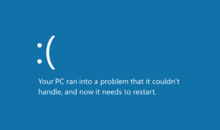
\includegraphics[width=\textwidth]{graphics/Pic/day 2/220px-Blue_Screen_of_Death.png}
    \caption{BlueScreenOfDeath}
    \label{fig:image}
  \end{minipage}
  \hfill
  \begin{minipage}[b]{0.3\textwidth}
    \centering
    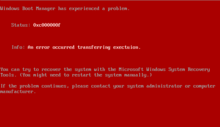
\includegraphics[width=\textwidth]{graphics/Pic/day 2/220px-Red_Screen_of_Death.png}
    \caption{Red Screen of Death}
    \label{fig:image_two}
  \end{minipage}
  \vfill
  \begin{minipage}[b]{0.3\textwidth}
    \centering
    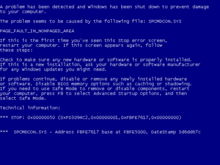
\includegraphics[width=\textwidth]{graphics/Pic/day 2/220px-Windows_XP_BSOD.png}
    \caption{Windows XP BSOD}
    \label{fig:image_three}
  \end{minipage}
  \hfill
  \begin{minipage}[b]{0.3\textwidth}
    \centering
    
\includegraphics[width=\textwidth]{graphics/Pic/day 2/Windows11BSOD.jpg}
    \caption{Windows11 BSOD}
    \label{fig:image_four}
  \end{minipage}
  \caption{BSOD?}
  \label{fig:images_img}
\end{figure}

\pagebreak

\section{Hintergrund}

Der Blue Screen of Death (BSOD) erschien erstmals in frühen Versionen von Windows. Wenn das Betriebssystem auf schwerwiegende Fehler stieß, die es nicht beheben konnte, zeigte es eine Fehlermeldung im Textmodus an. In späteren Versionen, wie Windows 3.1, wurde diese Fehlermeldung auf einem blauen Hintergrund angezeigt. Die Einführung des BSOD in seiner heute bekannten Form erfolgte mit Windows NT.\cite{wikipedia}

BSODs können durch schlecht programmierte Gerätetreiber oder fehlerhafte Hardware verursacht werden, z.B. defekten Speicher, Probleme mit der Stromversorgung, Überhitzung oder Hardware, die außerhalb ihrer Spezifikationsgrenzen betrieben wird. Auch inkompatible DLLs oder Fehler im Betriebssystemkern können zu BSODs führen.\cite{avast}

\section*{Photos}
\begin{figure}[!ht]
  \centering
  \begin{minipage}[b]{0.4\textwidth}
    \centering
    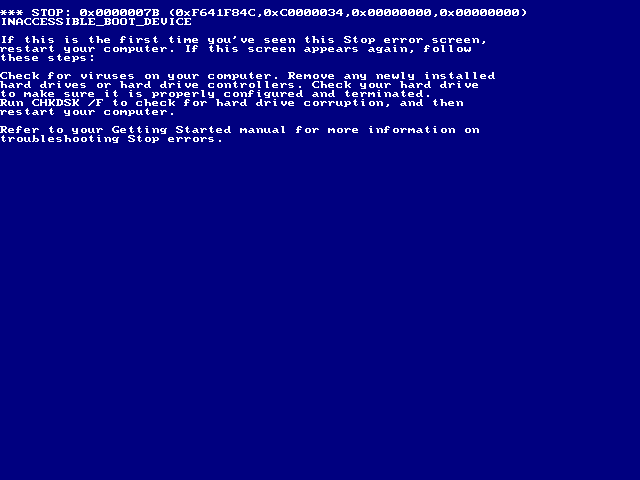
\includegraphics[width=\textwidth]{graphics/Pic/029-bsod_Windows_2000.png}
    \caption{Windows 2000}
    \label{fig:image1}
  \end{minipage}
  \hfill
  \begin{minipage}[b]{0.4\textwidth}
    \centering
    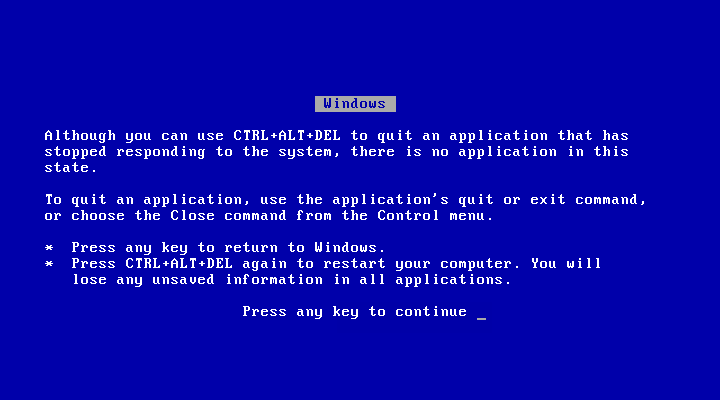
\includegraphics[width=\textwidth]{graphics/Pic/Windows_3.1_BSoD_(fixed).png}
    \caption{Windows 9x}
    \label{fig:image2}
  \end{minipage}
  \vfill
  \begin{minipage}[b]{0.4\textwidth}
    \centering
    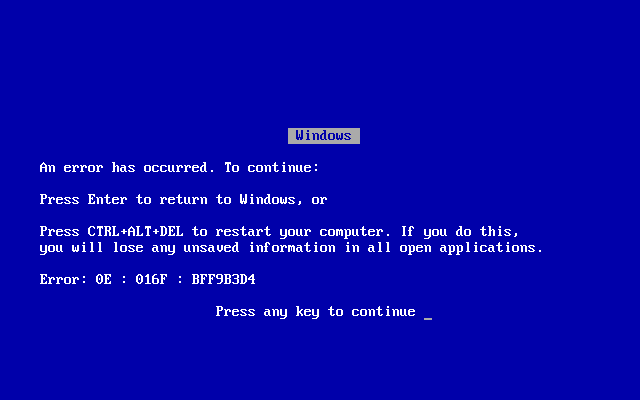
\includegraphics[width=\textwidth]{graphics/Pic/Windows_9X_BSOD.png}
    \caption{Windows Me}
    \label{fig:image3}
  \end{minipage}
  \hfill
  \begin{minipage}[b]{0.4\textwidth}
    \centering
    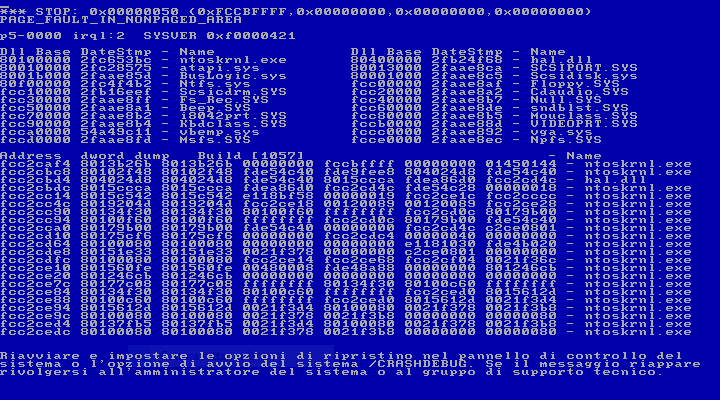
\includegraphics[width=\textwidth]{graphics/Pic/Windows_NT_3.51_BSOD_ita.png}
    \caption{Windows XP/Vista/7}
    \label{fig:image4}
  \end{minipage}
  \caption{BSOD-Staat im Laufe der Geschichte}
  \label{fig:images}
\end{figure}


\pagebreak
\section{Methode}

In diesem Abschnitt wird der spezifische Ansatz zur Analyse des Blue Screen of Death (BSOD) beschrieben. Dabei wird auf die verschiedenen Arten von BSODs und deren häufigsten Ursachen eingegangen, wobei zwischen Hardware- und Softwareproblemen unterschieden wird.

\subsection{Arten von BSODs}

Der BSOD kann in verschiedenen Formen auftreten, je nach zugrunde liegendem Problem. Die häufigsten Arten von BSODs sind:

\begin{itemize}
  \item \textbf{Stop-Fehler:} Diese Fehler treten auf, wenn das Betriebssystem einen schwerwiegenden Fehler entdeckt, von dem es sich nicht erholen kann. Typische Stop-Fehler-Codes sind z.B.
        \\\texttt{0x0000007B} (INACCESSIBLE\_BOOT\_DEVICE) oder \texttt{0x0000001E}
        \\(KMODE\_EXCEPTION\_NOT\_HANDLED).\cite{microsoft_support}
  \item \textbf{Treiberfehler:} Diese Fehler werden durch inkompatible oder fehlerhafte Gerätetreiber verursacht. Beispiele sind
        \\\texttt{0x000000D1} (DRIVER\_IRQL\_NOT\_LESS\_OR\_EQUAL) und \texttt{0x000000EA}
        \\(THREAD\_STUCK\_IN\_DEVICE\_DRIVER).\cite{malwarebytes}
  \item \textbf{Hardwarefehler:} Diese Fehler resultieren aus Problemen mit der Hardware, wie z.B. defektem RAM, fehlerhaften Festplatten oder überhitzten Komponenten. Beispiele sind \texttt{0x0000009C} (MACHINE\_CHECK\_EXCEPTION) und \texttt{0x00000050} (PAGE\_FAULT\_IN\_NONPAGED\_AREA).
  \item \textbf{Windows 11: Black Screen of Death?} In Windows 11 ist der BSOD größtenteils schwarz, außer dem blauen QR-Code, aber die Meldung ist im Wesentlichen dieselbe wie in früheren Versionen.\cite{microsoft_forum}
\end{itemize}

\subsection{Ursachenanalyse}

Die Ursachenanalyse eines BSODs erfordert ein systematisches Vorgehen, um die genaue Quelle des Problems zu identifizieren. Der Prozess umfasst folgende Schritte:

\begin{enumerate}
  \item \textbf{Fehlermeldung und Codes analysieren:} Die auf dem BSOD angezeigten Fehlercodes und Meldungen geben erste Hinweise auf die Ursache des Problems. Diese Informationen sollten notiert und in einschlägigen Datenbanken oder Dokumentationen nachgeschlagen werden.
  \item \textbf{Ereignisprotokolle überprüfen:} Das Windows-Ereignisprotokoll enthält detaillierte Informationen über Systemereignisse und Fehler. Durchsuchen Sie das Protokoll nach kritischen Ereignissen, die zeitlich mit dem Auftreten des BSODs übereinstimmen.\cite{wikipedia}
  \item \textbf{Treiber und Hardware testen:} Führen Sie Tests durch, um mögliche Hardwarefehler zu identifizieren, z.B. durch Überprüfen des RAMs mit \texttt{memtest86+} oder der Festplatten mit dem \texttt{chkdsk}-Befehl. Aktualisieren Sie Gerätetreiber oder installieren Sie sie neu, um Treiberprobleme auszuschließen.
  \item \textbf{Diagnosetools verwenden:} Nutzen Sie spezialisierte Diagnosetools wie den Windows Debugger (\texttt{WinDbg}) und das BlueScreenView-Tool, um detaillierte Informationen aus den Speicherabbilddateien (\texttt{.dmp}-Dateien) zu extrahieren und die Ursache des BSODs zu bestimmen.\cite{microsoft_support}
\end{enumerate}

\subsection{Häufigste Ursachen für BSOD}

Die häufigsten Ursachen für einen Blue Screen of Death auf Ihrem Windows-PC sind:

\begin{itemize}
  \item \textbf{Treiber:} Laut Microsoft sind 70\% der Blue Screen of Death-Fehlermeldungen auf veraltete oder inkompatible Treiber zurückzuführen, die zu Konflikten im System führen können.\cite{microsoft_support}
  \item \textbf{Software:} Inkompatible Software wie Apps oder Programme können Konflikte verursachen, die zu einem BSOD führen.\cite{malwarebytes}
  \item \textbf{Hardware:} Fehlerhafter Speicher (RAM), Festplatten (HDD), Solid-State-Laufwerke (SSD), Mainboards, Prozessoren oder Netzteile (PSU) können alle für Blue Screen-Abstürze verantwortlich sein.\cite{microsoft_forum}
  \item \textbf{Überhitzung:} Ihr Computer kann den BSOD anzeigen, wenn er aufgrund von Staub, defekten Lüftern oder überlasteter Hardware überhitzt.\cite{avast}
  \item \textbf{Malware:} Malware, wie ein PC-Virus, der Ihre wichtigen Dateien und Ordner beschädigt, kann der Grund für einen Blue Screen of Death sein.\cite{malwarebytes}
\end{itemize}

\subsection{Verwaltung des BSOD in Windows}

Wir können verhindern, dass Windows nach einem Blue Screen-Fehler automatisch neu startet, indem wir folgende Schritte ausführen:
\begin{itemize}
  \item Geben wir in der Windows -Suchleiste „Systemeigenschaften“ ein und drücken wir Enter.
  \item Suchen wir im Tab „Erweitert“ nach „Starten und Wiederherstellen“.
  \item Klicken auf Einstellungen und deaktivieren Sie die Option „Automatisch neu starten“ unter Systemfehler, um zu verhindern, dass Ihr PC nach dem BSOD automatisch neu startet.
  \item Hier können Sie auch festlegen, wie Windows ein Systemfehlerereignis im Systemprotokoll speichert.\cite{microsoft_support}
\end{itemize}

\section{Evaluation}

In diesem Abschnitt werden der vorgeschlagene Ansatz zur Analyse und Behebung des Blue Screen of Death (BSOD) mit anderen bestehenden Ansätzen verglichen und die Vor- und Nachteile der verschiedenen Methoden zur Diagnose und Lösung von BSOD-Problemen diskutiert.

\subsection{Vergleich des Lösungsansatzes mit anderen bestehenden Ansätzen}

Der vorgeschlagene Ansatz zur Diagnose und Behebung von BSOD-Problemen umfasst die systematische Analyse von Fehlercodes, die Überprüfung von Ereignisprotokollen, das Testen von Treibern und Hardware sowie die Nutzung spezialisierter Diagnosetools. Dieser Ansatz wird nun mit anderen bestehenden Methoden verglichen:

\begin{itemize}
  \item \textbf{Manuelle Fehlersuche:} Traditionell wird die manuelle Fehlersuche verwendet, bei der Administratoren oder Techniker die auf dem BSOD angezeigten Fehlercodes und Meldungen untersuchen und in Dokumentationen nachschlagen. Diese Methode kann zeitaufwändig und fehleranfällig sein, erfordert jedoch keine speziellen Tools.
  \item \textbf{Automatisierte Diagnosetools:} Es gibt verschiedene automatisierte Tools wie BlueScreenView, WhoCrashed und Windows Debugger (WinDbg), die detaillierte Informationen aus Speicherabbilddateien extrahieren und mögliche Ursachen identifizieren können. Diese Tools können die Diagnose beschleunigen und genaue Informationen liefern, sind jedoch oft komplex in der Handhabung.\cite{microsoft_support}
  \item \textbf{Proaktive Wartung:} Einige Ansätze setzen auf proaktive Wartung, bei der regelmäßig Treiber und Software aktualisiert, Hardwarekomponenten überprüft und Systemressourcen überwacht werden, um BSODs zu verhindern. Dies erfordert kontinuierliche Aufmerksamkeit und Ressourcen, kann jedoch dazu beitragen, Ausfälle zu minimieren.\cite{microsoft_forum}
\end{itemize}

\subsection{Diskussion der Vor- und Nachteile der verschiedenen Methoden}

Jede der genannten Methoden zur Diagnose und Behebung von BSOD-Problemen hat ihre eigenen Vor- und Nachteile:

\begin{itemize}
  \item \textbf{Manuelle Fehlersuche:}
        \begin{itemize}
          \item \textbf{Vorteile:} Keine speziellen Tools erforderlich, flexibel anwendbar.\cite{microsoft_forum}
          \item \textbf{Nachteile:} Zeitaufwändig, fehleranfällig, erfordert Expertenwissen.\cite{avast}
        \end{itemize}
  \item \textbf{Automatisierte Diagnosetools:}
        \begin{itemize}
          \item \textbf{Vorteile:} Schnelle und genaue Diagnose, detaillierte Informationen, erleichtert die Fehlersuche.\cite{microsoft_support}
          \item \textbf{Nachteile:} Komplex in der Handhabung, erfordert Schulung und Verständnis der Tools.\cite{malwarebytes}
        \end{itemize}
  \item \textbf{Proaktive Wartung:}
        \begin{itemize}
          \item \textbf{Vorteile:} Kann BSODs vorbeugen, verbessert die Systemstabilität, reduziert Ausfallzeiten.\cite{avast}
          \item \textbf{Nachteile:} Erfordert kontinuierliche Aufmerksamkeit und Ressourcen, nicht immer effektiv bei unvorhersehbaren Fehlern.\cite{microsoft_forum}
        \end{itemize}
\end{itemize}

\subsection{Wie behebt man einen Blue Screen of Death?}

Ein gelegentlicher BSOD, den Sie nie wieder sehen, könnte harmlos sein. Regelmäßige Blue Screens können jedoch problematisch und frustrierend sein, da sie auf tiefere Probleme hinweisen und dazu führen können, dass Sie bei jedem Neustart Daten verlieren. Nach einem BSOD sind zwei Dinge zu beachten:

\begin{itemize}
  \item Softwareprobleme aufgrund von schlechtem Code, Inkompatibilität oder Malware.\cite{microsoft_support}
  \item Hardwareprobleme aufgrund von Inkompatibilität oder Schäden durch Stöße, Alterung oder Spannungsfluktuationen.\cite{avast}
\end{itemize}

\textbf{Treiber:} Geben Sie „Nach Updates suchen“ in die Windows-Suchleiste ein, um Windows Update zu finden. Verwenden Sie diese Funktion, um Ihre Treiber und Software zu aktualisieren und die Stabilität zu verbessern. Neue Treiber können jedoch selten auch Systemfehler verursachen. Sie könnten versuchen, die Änderungen zurückzusetzen, wenn ein neuer Treiber BSOD-Probleme ausgelöst hat.

\textbf{Schlechte Software:} Software, die nicht gut mit anderen Programmen harmoniert, kann Blue Screen Abstürze verursachen. Jede kürzlich heruntergeladene oder installierte Software könnte der Schuldige sein. Geben Sie „Programme hinzufügen oder entfernen“ in die Windows-Suchleiste ein, um die Einstellung „Apps und Features“ zu finden. Deinstallieren Sie hier die verdächtigen Programme. Sie können auch den abgesicherten Modus von Windows verwenden, wenn Sie aufgrund von Blue Screen Fehlern keine Software normal entfernen können.\cite{avast}

Alternativ können Sie die Systemwiederherstellungsfunktion verwenden, wenn Ihr Computer über Wiederherstellungspunkte verfügt. Geben Sie „Wiederherstellung“ in die Windows-Suchleiste ein und starten Sie die „Erweiterte Wiederherstellungstools“ aus der Systemsteuerung. Klicken Sie auf „Systemwiederherstellung öffnen“, um Ihr System auf einen potenziell stabileren Zustand zurückzusetzen.\cite{microsoft_support}

\textbf{Malware:} Viele verschiedene Arten von Malware, wie Computerviren, Computerwürmer, einige Trojaner und Ransomware, können einen BSOD verursachen, indem sie Ihre wichtigen Dateien beschädigen. Verwenden Sie einen kostenlosen Virus- und Malware-Scanner, um alle Arten von Malware zu finden und zu entfernen, um Ihr System zu reinigen.\cite{malwarebytes}

\textbf{Peripheriegeräte und neue Hardware:} Entfernen Sie alle Peripheriegeräte, die den BSOD verursachen könnten. Beginnen Sie damit, Drucker, Scanner, USB-Geräte und externe Speicher von Ihrem PC zu trennen. Entfernen Sie anschließend alle neuen Hardwarekomponenten. Wenn Sie beispielsweise einen neuen RAM-Riegel gekauft haben, verwenden Sie den alten. Wenn Sie eine neue Grafikkarte gekauft haben, wechseln Sie zurück zur vorherigen oder verwenden Sie die integrierten Grafikoptionen.\cite{microsoft_forum}

Wenn nach dem Entfernen der nicht wesentlichen Hardware keine Blue Screen Fehler mehr auftreten, fügen Sie die Hardware nacheinander wieder hinzu, um das Problem zu isolieren. Panik ist nicht notwendig, wenn eine neue Hardware BSODs verursacht, da sie möglicherweise nicht fehlerhaft ist. Beispielsweise ist Ihr neuer RAM-Riegel möglicherweise nicht mit Ihrem Mainboard oder Ihrem anderen RAM-Riegel kompatibel. Ebenso kann eine perfekte Grafikkarte aufgrund von Konflikten, Treiberproblemen oder unzureichender Stromversorgung Abstürze verursachen.\cite{avast}

\textbf{Hardwaretests:} Sie können Ihren Speicher mit Windows- oder Drittanbieter-Tools auf Fehler überprüfen. HCI Designs MemTest ist ein beliebtes Tool für RAM-Tests. Suchen Sie alternativ nach „Windows-Speicherdiagnose“ in der Windows 10 Suchleiste.

Verwenden Sie die Software Ihres Speicherlaufwerkherstellers, um Ihre Festplatte (HDD) oder Solid-State-Laufwerk (SSD) auf Fehler zu überprüfen. Hier sind einige schnelle Links für Samsung, Western Digital und Seagate.

Achten Sie auf Artefakte oder langsame Computerreaktionen beim Spielen von Videospielen, um zu sehen, ob Ihre GPU fehlerhaft ist. Sie können auch Videospiel-Benchmarking-Tools verwenden, um Ihre Grafikkarte auf Defekte zu überprüfen.\cite{microsoft_support}

Ein fehlerhaftes Netzteil kann dazu führen, dass Ihr Computer überhitzt, spontan neu startet, langsamer wird, abstürzt oder den BSOD anzeigt. Die einfachste Möglichkeit, ein Netzteil zu testen, besteht darin, ein neues auszuprobieren.

Überhitzung kann Blue Screen Fehler verursachen. Sie können ein Dienstprogramm wie Open Hardware Monitor verwenden, um die Temperaturen Ihrer CPU und GPU zu überprüfen. Ein Druckluftspray kann die Lüftungsschlitze und Lüfter in einem überhitzten Computer reinigen. Ihr System sollte auch gut belüftet sein, um kühl zu bleiben.\cite{microsoft_support}

\pagebreak
\section{Fehlermeldungen in anderen Farben}

In diesem Abschnitt werden verschiedene Fehlermeldungen untersucht, die in unterschiedlichen Betriebssystemen und Softwareumgebungen auftreten können und durch verschiedene Farben gekennzeichnet sind.\cite{wikipedia}

\subsection{Windows 11 Schwarzer Bildschirm des Todes}

Mit der Einführung von Windows 11 hat Microsoft zeitweise eine Änderung der bekannten Blue Screen of Death (BSOD) in eine schwarze Version vorgenommen. Diese Änderung sollte visuell besser zum neuen Design von Windows 11 passen, wurde jedoch später wieder zurückgenommen, sodass der Bildschirm nun wieder blau erscheint. Die Änderung betraf hauptsächlich die Darstellung und hatte keine Auswirkungen auf die Ursachen oder die Lösung von Systemfehlern. Ein Beispiel für diese Änderung findet sich in der Insider Preview Version von Windows 11, wo Benutzer die neue Farbe des Fehlerbildschirms berichteten.\cite{microsoft_forum,warren2021,windows_insider2021}

\subsection{MS-DOS 6 Schwarzer Bildschirm des Todes}

In älteren Betriebssystemen wie MS-DOS 6 war der „Schwarze Bildschirm des Todes“ eine häufige Erscheinung. Dieser Fehler trat auf, wenn ein schwerwiegender Systemfehler, wie ein Prozessor-Interrupt im geschützten Modus, erkannt wurde. Anders als bei Windows gab es bei MS-DOS keine grafische Oberfläche zur Fehleranzeige, und der Fehler wurde im Textmodus dargestellt. Solche Fehler erforderten oft einen kompletten Neustart des Systems und waren ein frühes Beispiel für kritische Systemabstürze in der Computerwelt.

\subsection{Windows 3.x Schwarzer Bildschirm des Todes}

Bei Windows 3.x trat ein schwarzer Bildschirm auf, wenn eine MS-DOS-Anwendung nicht korrekt ausgeführt wurde, oft verursacht durch aktive Netzwerktreiber. Diese Art von Fehler führte dazu, dass der Bildschirm in den Textmodus wechselte, jedoch keine Inhalte anzeigte. Solche Fehler erforderten ebenfalls einen Neustart des Systems und stellten eine Herausforderung für die Benutzer dar, da keine detaillierten Fehlerinformationen bereitgestellt wurden.

\subsection{Xbox 360 Schwarzer Bildschirm des Todes}

Auf der Xbox 360 konnte ein schwarzer Bildschirm angezeigt werden, wenn das System auf einen schwerwiegenden Fehler stieß. Diese Fehlermeldung forderte die Benutzer auf, den Xbox-Support zu kontaktieren und zeigte einen spezifischen Fehlercode (z. B. E71 oder E64) an. Zusätzlich leuchtete ein Viertel des Rings um den Einschaltknopf rot auf, was den „Red Ring of Death“ signalisierte und auf einen Hardwarefehler hinwies.

\subsection{OS/2 Schwarzer Bildschirm des Todes}

Das Betriebssystem OS/2 zeigte bei kritischen Fehlern ebenfalls einen schwarzen Bildschirm an. Dieser Bildschirm, auch als TRAP-Bildschirm bekannt, wurde angezeigt, wenn ein nicht behebbarer Fehler im Kernel auftrat. Der Bildschirm zeigte detaillierte Informationen über den Fehler, einschließlich Prozessorregister und Stack, und ermöglichte es dem Benutzer, das System neu zu starten oder Speicherinformationen zu speichern.

\subsection{Roter Bildschirm des Todes}

Ein „Roter Bildschirm des Todes“ (RSoD) wurde in einigen Beta-Versionen von Windows Vista verwendet. Diese Art von Fehlerbildschirm wurde verwendet, um besonders schwerwiegende Fehler darzustellen. Obwohl er in der finalen Version von Vista nicht mehr verwendet wurde, bleibt er ein bemerkenswertes Beispiel für die Darstellung von Systemfehlern in verschiedenen Farben.

\subsection{Andere Verwendungen}

Farbcodierte Fehlermeldungen werden auch in anderen Kontexten verwendet:
\begin{itemize}
  \item \textbf{Flugsimulatoren:} In einigen Flugsimulatoren werden bei simulierten Abstürzen alle Bildschirme im Cockpit rot angezeigt, um einen kritischen Fehler darzustellen.
  \item \textbf{PlayStation 2:} Ein roter Bildschirm erscheint, wenn eine nicht unterstützte oder beschädigte Disk eingelegt wird, mit der Meldung, eine kompatible DVD/CD-ROM einzulegen.\cite{wikipedia}
  \item \textbf{PlayStation Portable:} Ein roter Bildschirm kann auftreten, wenn der interne Flash-Speicher beschädigt ist.
  \item \textbf{SEGA Genesis / Mega Drive:} Ein fehlerhaft gepatchtes ROM kann einen roten Bildschirm ohne Text anzeigen, der nur durch einen Neustart der Konsole behoben werden kann.
\end{itemize}

\pagebreak
\subsection{Tabellen}
\begin{table}[!ht]
  \centering
  \begin{tabular}{|l|l|p{3.5cm}|p{3.5cm}|}
    \hline
    \textbf{Fehlermeldung} & \textbf{Betriebssystem} & \textbf{Ursache}                  & \textbf{Lösung}                            \\ \hline
    Blue Screen of Death   & Windows 10              & Hardwarefehler, Treiberprobleme   & Neustart, Treiberaktualisierung            \\ \hline
    Black Screen of Death  & Windows 11              & Systemabsturz, BIOS-Einstellungen & BIOS zurücksetzen, Systemwiederherstellung \\ \hline
    Red Screen of Death    & Windows Vista           & Systemfehler in Betaversionen     & Betaversion aktualisieren                  \\ \hline
    Kernel Panic           & Linux                   & Fehler im Kernel, Hardwarefehler  & Systemneustart, Kernel-Debugging           \\ \hline
    Guru Meditation        & AmigaOS                 & Fehler im Betriebssystem          & Neustart                                   \\ \hline
  \end{tabular}
  \caption{Übersicht der Systemfehler und deren Ursachen}
  \label{table:system_errors}
\end{table}


\begin{table}[!ht]
  \centering
  \begin{tabular}{|l|p{2.5cm}|p{3.5cm}|p{3.5cm}|}
    \hline
    \textbf{Betriebssystem} & \textbf{Fehlertyp}    & \textbf{Durchschnittliche Wiederherstellungszeit} & \textbf{Maximale Wiederherstellungszeit} \\ \hline
    Windows 10              & Blue Screen of Death  & 5 Minuten                                         & 20 Minuten                               \\ \hline
    Windows 11              & Black Screen of Death & 10 Minuten                                        & 30 Minuten                               \\ \hline
    Windows Vista           & Red Screen of Death   & 15 Minuten                                        & 45 Minuten                               \\ \hline
    Linux                   & Kernel Panic          & 8 Minuten                                         & 25 Minuten                               \\ \hline
    AmigaOS                 & Guru Meditation       & 3 Minuten                                         & 10 Minuten                               \\ \hline
  \end{tabular}
  \caption{Vergleich der Wiederherstellungszeiten bei verschiedenen Fehlertypen}
  \label{table:recovery_times}
\end{table}

\pagebreak
\subsection*{Plots}
\begin{figure}[!ht]
  \centering
  \begin{minipage}[b]{0.4\textwidth}
    \centering
    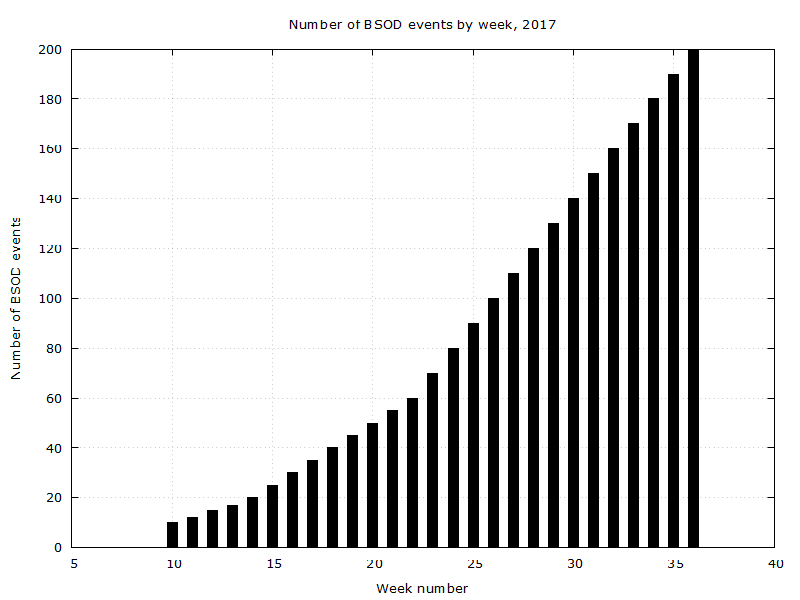
\includegraphics[width=\textwidth]{graphics/Charts/New_Charts/plot1.png}
    \caption{Number of BSOD events per week}\cite{mosaic2017}
    \label{fig:Plot1}
  \end{minipage}
  \hfill
  \begin{minipage}[b]{0.4\textwidth}
    \centering
    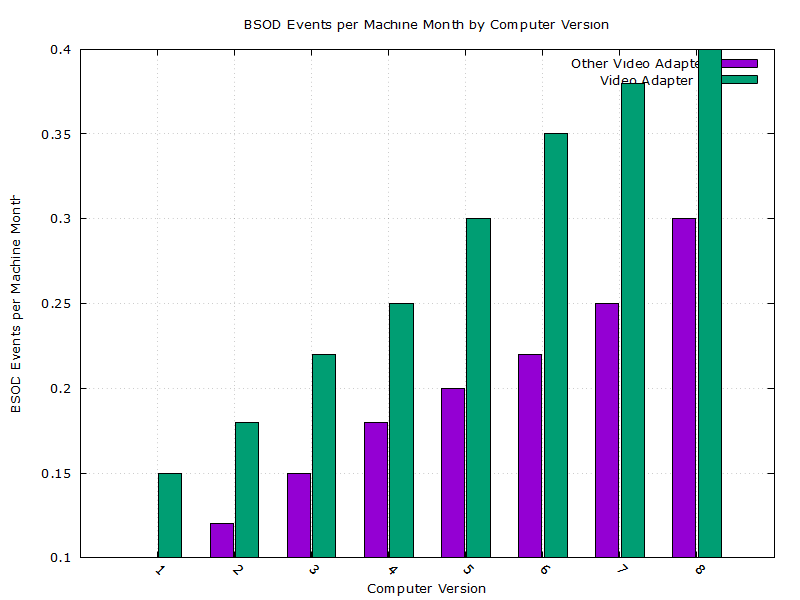
\includegraphics[width=\textwidth]{graphics/Charts/New_Charts/plot2.png}
    \caption{BSOD events per month in most common computer versions.}\cite{mosaic2017}
    \label{fig:Plot2}
  \end{minipage}
  \vfill
  \begin{minipage}[b]{0.4\textwidth}
    \centering
    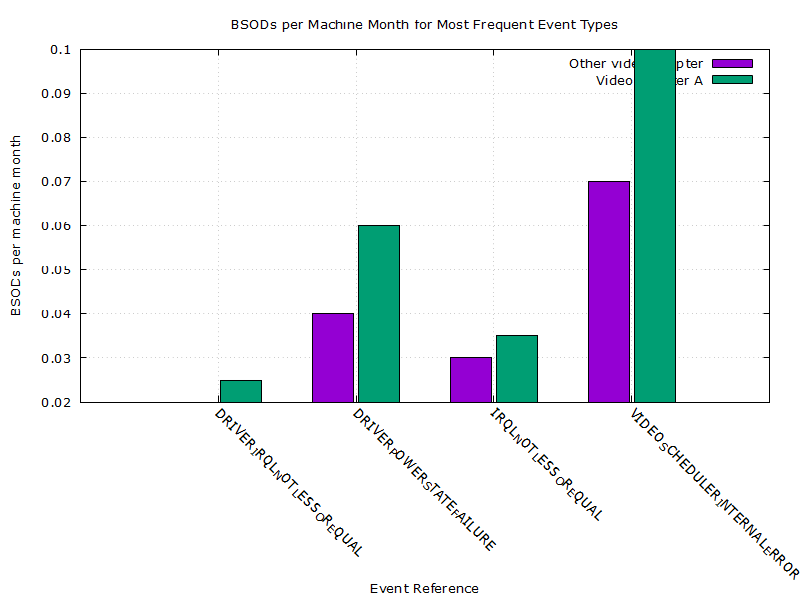
\includegraphics[width=\textwidth]{graphics/Charts/New_Charts/plot3.png}
    \caption{ BSOD events per month for most common BSOD types}\cite{mosaic2017}
    \label{fig:Plot3}
  \end{minipage}
  \label{fig:Plots}
\end{figure}
\pagebreak
\section{Fazit}

In diesem Bericht wurde die Problematik des Blue Screen of Death (BSOD) analysiert und verschiedene Ansätze zur Diagnose und Behebung dieser Probleme untersucht. Die wichtigsten Ergebnisse lassen sich wie folgt zusammenfassen:

Der \textbf{Blue Screen of Death (BSOD)} ist ein gefürchteter Fehlerbildschirm, den Windows anzeigt, wenn etwas schwerwiegend schiefläuft. Man könnte es als den letzten Ausweg des Betriebssystems bezeichnen, wenn es einen Fehler nicht selbst beheben kann. Statt weiterzumachen und möglicherweise noch mehr Schaden anzurichten, schaltet der Computer komplett ab und zeigt den blauen Bildschirm mit einigen technischen Details an.\cite{WindowsInternalsPart1}

\subsection*{Wie der BSOD dein System beeinträchtigt}

\begin{itemize}
  \item \textbf{Alles stoppt}: Wenn ein BSOD auftritt, bleibt dein Computer plötzlich stehen. Nichts reagiert mehr, und du kannst nur noch den Reset-Knopf drücken. Das System macht das, um zu verhindern, dass noch mehr kaputtgeht.\cite{WindowsInternalsPart1,WindowsInternalsPart2}
  \item \textbf{Datenverlust}: Wenn du gerade an etwas gearbeitet hast und nicht gespeichert hast, ist es höchstwahrscheinlich verloren. Dateien, die du gerade bearbeitet hast, könnten beschädigt sein, und du musst sie möglicherweise wiederherstellen.\cite{WindowsInternalsPart1,WindowsInternalsPart2}
  \item \textbf{Neustart und Fehlersuche}: Nach einem BSOD startet der Computer normalerweise neu. Windows versucht dann, herauszufinden, was schiefgelaufen ist. Wenn der BSOD häufiger auftritt, kann das ein Hinweis auf ernstere Probleme wie kaputte Hardware oder inkompatible Software sein.\cite{WindowsInternalsPart1,WindowsInternalsPart2}
  \item \textbf{Zuverlässigkeit des Systems}: Wenn der BSOD öfter passiert, wird dein Computer unzuverlässig. Das kann besonders ärgerlich sein, wenn du mitten in einer wichtigen Arbeit bist. In einem Unternehmen kann das zu Ausfallzeiten führen und wichtige Arbeitsprozesse stören.\cite{WindowsInternalsPart1,WindowsInternalsPart2}
\end{itemize}

Die verschiedene Punkte die Im Bericht bescprochen werden
\begin{itemize}
  \item Verschiedene Diagnosemethoden, einschließlich manueller Fehlersuche, automatisierter Diagnosetools und proaktiver Wartung, bieten unterschiedliche Vor- und Nachteile bei der Identifizierung und Lösung von BSOD-Problemen.\cite{microsoft_support}
  \item Die Evaluation ergab, dass automatisierte Diagnosetools wie BlueScreenView und WinDbg eine schnelle und präzise Fehlerdiagnose ermöglichen, während proaktive Wartungsansätze zur Vorbeugung von BSODs beitragen können, jedoch kontinuierliche Überwachung erfordern.\cite{microsoft_support}
  \item Es wurde auch diskutiert, wie Nutzer durch einfache Schritte wie Treiberaktualisierungen, Softwarebereinigung und Hardwaretests die Wahrscheinlichkeit von BSODs reduzieren können.\cite{avast}
\end{itemize}

Als mögliche nächste Schritte zur Verbesserung der BSOD-Diagnose und -Behebung könnten weitere Forschungen in folgenden Bereichen angestrebt werden:

\begin{itemize}
  \item Entwicklung fortschrittlicher Diagnosetools, die auch für nicht-technische Benutzer zugänglich sind.
  \item Integration von Künstlicher Intelligenz und maschinellem Lernen zur automatisierten Analyse von BSOD-Fehlern.
  \item Stärkere Zusammenarbeit zwischen Hardwareherstellern, Softwareentwicklern und Sicherheitsexperten, um die Stabilität und Kompatibilität von Systemkomponenten zu verbessern.
  \item Förderung von Bildungsprogrammen und Bewusstseinskampagnen, um Anwender über beste Praktiken bei der Vermeidung und Behebung von BSOD-Problemen aufzuklären.\cite{microsoft_support}
\end{itemize}

Kurz gesagt: Der Blue Screen of Death ist nicht nur nervig, sondern kann ernsthafte Folgen haben, vor allem wenn man die Ursache nicht schnell in den Griff bekommt.


% Hier beginnt das Literaturverzeichnis
\clearpage
\renewcommand\refname{Literaturverzeichnis}
\bibliographystyle{alpha}
\bibliography{literatur}
\addcontentsline{toc}{section}{Literaturverzeichnis}
% Hier beginnt der Anhang
\clearpage
\appendix
\part*{Anhang}
\addcontentsline{toc}{section}{Anhang}
\section{Quellen}
\href{https://commons.wikimedia.org/wiki/BSoD?uselang=de}{All pictures used are in Wiki Commons}\cite{wikicommons_bsod}\\
\href{https://mosaicdatascience.com/2017/11/30/diagnosing-windows-10-crashes-predictive-ai-services/}{Plots are from Mosaic DataScience}\cite{mosaic2017}\\
\href{https://www.amazon.de/-/en/Pavel-Yosifovich/dp/0735684189}{The Windows Internals, Part 1, 7th Edition is available on Amazon}\cite{WindowsInternalsPart1}\\
\href{https://www.amazon.de/-/en/Mark-Russinovich/dp/0135462401}{The Windows Internals, Part 2, 7th Edition is available on Amazon}\cite{WindowsInternalsPart2}
\end{document}
